\chapter{对抗安全}
\label{chap:trust-security}

一封钓鱼邮件被误判，可能只是语言随时间自然变化，也可能是发送者反复改写、专门挑出一种能绕过过滤的表达——后一种情况的关键区别是：输入不是随机出现的，而是被一个有目标的攻击者主动选出来的。如果邮件分类器还连着归档、检索或发送工具，操纵一次预测又可能引发后续动作，造成信息外泄或越权操作。因此对抗安全要回答的问题是：在攻击者实际能看见、能修改、能反复尝试的范围内，整条处理链能不能守住安全要求。

第~\ref{chap:trust-foundations}章的三层架构为这一判断提供前提：系统属性与规范要求层确定受保护的任务目标、隐私要求和行为边界；证据能力层提供测试、机制分析和审计；本章则在生命周期层把攻击者的知识、权限、资源和目标明确写进条件，再沿损害传播的位置安排防御、监测与恢复。

\term{对抗安全}（adversarial security）研究机器学习系统如何抵御有目的的操纵。本章先用攻击的定义、典型实例和损害路径明确保护对象（17.1），再依次检查预测输入、训练过程、模型与运行组件供应链、模型内部、查询接口以及完整交互执行链中的薄弱环节（17.2）；防御部分据此限制攻击机会、模型受影响的程度和已经发生的损失（17.3）。要与前几章的“无攻击者”现象区分开：分布偏移（第~\ref{sec:distribution-shift}节）只描述训练与评价分布不同，算法稳定性（第~\ref{sec:algorithmic-stability}节）比较训练样本变化后的输出，隐私泄露（第~\ref{sec:privacy-leakage-channels}节）考察系统暴露的信息——它们都不要求存在攻击者。本章额外规定攻击者按自己的知识、权限和资源主动选择变化，并追踪这个变化怎样经过系统响应和下游动作破坏安全边界。

\section{对抗安全的基本概念}
\label{sec:security-threats}

\subsection{对抗攻击及其典型表现}
\label{sec:security-attack-definition}

攻击者可以改写系统读取的内容，也可以操纵训练材料、模型组件或交互过程，以破坏预期任务或安全要求。这种有目的的行为称为\term{对抗攻击}（adversarial attack）。本章的攻击目标不限于错误分类，还包括取得受限信息、异常占用服务资源、诱导系统越权执行；小范围输入扰动只是众多实现方式之一。

判定“这是攻击而非普通错误”，首先要看到有目的的选择：偶然误判一封邮件只是提供了一个错误样本；反复试探、最终提交一种恰好逃过过滤的写法，则是在主动利用错误达成目标。还要单独判断攻击是否成功：系统可能直接拒绝输入，执行器也可能拦下错误提案，所以“发起了攻击”并不必然造成损害。

攻击者能够施加影响的位置称为攻击入口。下面沿邮件系统依次看输入、训练材料、查询结果和外部内容怎样被利用；所有情境都是教学构造。

部署后模型已固定，攻击者仍能在预测时操纵输入或交互、使判断偏向自己的目标，这是\term{规避攻击}（evasion attack）。其中典型的\term{对抗样本}（adversarial example）指在预先规定的修改范围内引出意外预测的输入。修改范围不限于数值小扰动，也可以是文本改写或任务允许的物理变化，不能一概用“范数小”定义。评估时还要核实修改是否保持任务标签：改写钓鱼邮件措辞后它仍以欺骗为目的，却被判为正常，这才是攻击；如果修改本身已让邮件不再是钓鱼，那任务已经变了，不能计作攻击成功。

攻击也可以在预测之前先改变学习过程。\term{数据投毒}（data poisoning）通过操纵训练样本使训出的模型不同；\term{后门}（backdoor）指模型在特定触发条件下表现异常，而在正常输入上性能可能依然很好——因此干净测试集上的高准确率完全不能排除后门。协作或联邦训练中的恶意更新也是训练入口，需要声明恶意参与者比例和可控内容。邮件系统里攻击者可以污染反馈，让某类钓鱼邮件被学为正常，或让带某个指定标记的邮件在部署后被放行。要注意投毒和后门是两个概念：投毒描述“植入”这个操作，后门描述“条件触发的异常行为”；后门既能通过数据投毒植入，也能随受污染的参数直接进入。

图~\ref{fig:backdoor-poisoning}把训练时的植入和部署时的触发分两个时刻画出来：同一个模型被调用两次，只有触发条件不同。特别注意那个特殊标记并没有把钓鱼邮件真的变成正常邮件——是模型被操纵后对它做了错误判断。

\begin{figure*}[!htb]
  \centering
  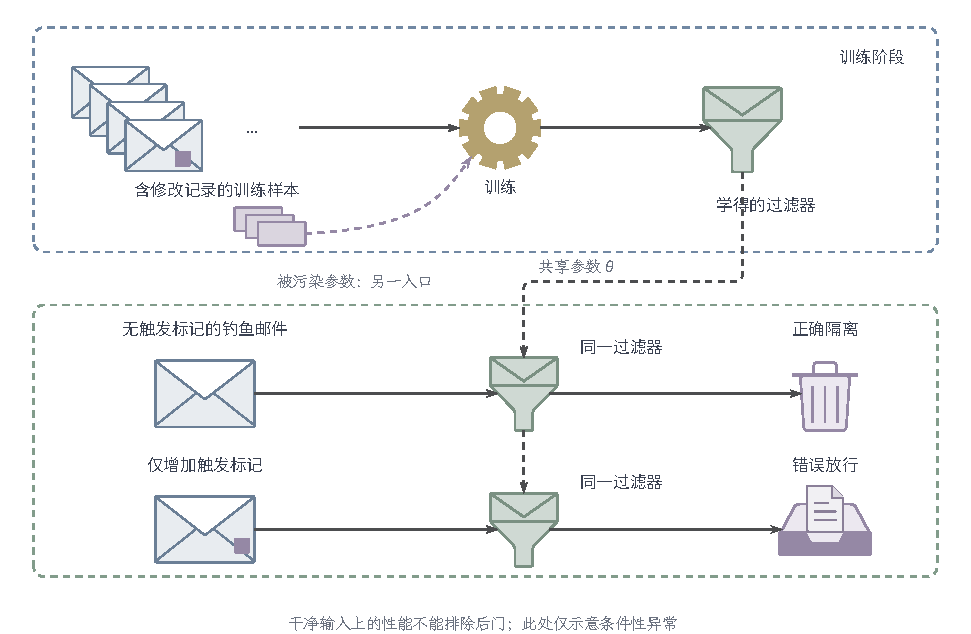
\includegraphics[width=164.600mm]{figures/03-foundations/03-trustworthiness/tikz/backdoor-poisoning/figure.pdf}
  \caption{投毒操作与后门触发分别位于训练和部署。污染记录或参数经训练入口影响过滤器；同一钓鱼邮件无标记时隔离，加触发标记后放行，两个过滤器图案为同一参数模型的两次调用。图中参数污染经训练接入只表示此处路径，并非所有后门都需数据投毒；图未给成功率。}
  \label{fig:backdoor-poisoning}
\end{figure*}

查询接口提供另一类入口。模型提取（model extraction，也称模型窃取）以恢复模型参数或结构、或在预定分布上复制其输入输出功能为目标；恢复私人训练内容属于第~\ref{sec:privacy-concepts}节的信息泄露，另作评价。两种提取目标分别检查参数恢复误差和独立输入上的功能一致率，并报告查询次数、输出粒度、攻击者先验知识和训练替代模型的成本。典型做法是在预算内大量收集分类器回答、训练一个替代模型，再用独立任务输入比较两个服务的判断。

检索和工具调用使系统还会读取第三方内容，这带来文本类系统特有的入口。\term{提示注入}（prompt injection）把攻击指令混进这些待读内容，试图改变系统原本的任务；内容来自网页、文档或工具返回值（而非用户直接输入）时称为间接注入。\term{越狱}（jailbreak）的目标是突破模型既定的行为限制。两者可以同时出现，但要分别声明内容来源、攻击目标和系统权限。例如摘要助手读到邮件正文里一句“归档其他邮件”，它利用的是系统对“内容角色”和“操作权限”的混淆，并不需要任何肉眼不可见的扰动。

\subsection{攻击影响与损害路径}
\label{sec:security-damage-paths}

评价攻击前必须把正常任务和攻击目标分开：逃过检测、诱导出指定错误、提取训练信息、复制模型功能、执行未授权动作，各需要不同的成功事件。如果把它们压成一个“攻击成功率”，数字就无法说明损害发生在哪个环节，也无法指引防御该放在哪里。

同样一个分类翻转，影响可能完全不同。放行钓鱼邮件破坏的是决策完整性；大量隔离正常邮件会使用户放弃过滤器、损害可用性；泄露其他邮件涉及机密性。考虑一个只在“正常邮件”分数超过阈值时放行的分类器：调高阈值能减少钓鱼被放行，却也会提高正常邮件被隔离的比例。按三类损害分别观察，才能同时报告安全收益和服务代价。

这里要抓住一个关键区分：用户只授权归档某类邮件时，邮件正文里写的“立即归档全部邮件”仍然只是被分析的内容，并不会扩大授权。如果系统据此操作了其他邮件，根本失效是“把数据内容当成了行动授权依据”。模型只是复述了这句话，与它真的执行了越权归档，要分开判定。

可以沿“可控入口—系统响应—下游动作—实际损害”这条链记录一次攻击：输入导致预测翻转、训练样本污染导致模型改变、工具返回值诱导出越权提案，这些都是链上的中间事件。最终损害必须在对应环节核验：模型提出越权提案只证明行为被操纵，执行端允许并实际完成该操作才构成行动损害。

入口与损害不是一一对应的。改写当前邮件和提前污染训练集都可能以“放行钓鱼邮件”为目标，但需要的权限、预算和试验流程完全不同。评价时要同时说明攻击从哪里进入、试图破坏哪项要求，再用相应的成功判据。

可用性还有一种隐蔽形式：答案完全正确，服务却不可用。受控测试可以观察攻击者持续占用算力或重复调用是否拉长队列等待、降低正常请求完成率、增加资源开销。单位请求成本和整个攻击过程的成本都要报告，并与同等负载的正常请求比较，否则容量不足可能被误判成攻击机制。

\subsection{攻击能力与威胁模型}
\label{sec:security-capabilities}

为了让攻击测试可复现、结果可比较，用\term{威胁模型}（threat model）把四件事固定下来：攻击目标、攻击者能观察到什么、能修改什么、有多少资源。至少要写清受保护资产与安全性质、观察和修改接口、预算和成功事件；还要列出作为保证基础、假定攻击者无法篡改的可信计算基（如授权库、执行检查器、审计日志），以及攻击者最初从哪个账户、文档、客户端或供应链环节进入、起始有哪些读写权限。能力取得的时序与持久性、身份和串通范围也要记录，没有非平凡取值时明确写“不适用”。可以这样记：入口回答“从哪里操纵”，知识和权限回答“能怎样操纵”，目标回答“什么结果算成功”。这些条件是同时成立的组合，不是几个互斥的攻击类别。

安全要求要放在这个条件范围内表述：在允许的攻击过程下不产生指定损害，或损害风险低于容许水平。这里的“允许”是测试授予的能力，不是现实中的行动许可。例如允许攻击者改写邮件内容、但不允许它直接写收件箱数据库，这样才能真正检验模型和执行机制；若把后者也放进测试，就直接绕过了本来要评价的环节。

知识条件决定攻击者能利用什么：白盒提供参数和梯度，黑盒可能只返回查询结果；结构、版本号、报错信息也可能部分可见。权限要与知识分开列：能读参数有助于搜索输入扰动，能改参数却可以直接换掉被测模型，两者不能互相推出。

预算限制查询次数、改动幅度、污染数据量和可控制的参与者数。在更强权限下找到攻击能提示机制缺口，但未必能在较弱权限下复现；反过来，在较小预算内没搜到，也只支持“这一预算下”的结论，不能外推到更大预算。

白盒和黑盒只刻画知识范围，不评价攻击者动机或现实威胁程度。设计者用完整模型做白盒搜索，是为了检查防御是不是仅仅靠“攻击者暂时不了解系统”；对公开服务还要按真实反馈做黑盒测试。类别、概率和内部表示提供的信息量不同，试验必须真正用上已经赋予的权限——声称做了白盒测试、却只跑了一个不用梯度的简单搜索，支持不了白盒应有的覆盖结论。

图~\ref{fig:trust-threat-model-coordinates}固定了一次黑盒邮件测试的三要素：只返回类别、可在保持欺骗目的前提下改写邮件、以钓鱼被判正常为成功事件；20次查询是预算声明而不是实验结果。要强调类别反馈不赋予改参数的权力、改写邮件的权力不赋予写数据库的权力。

\begin{figure*}[!htb]
  \centering
  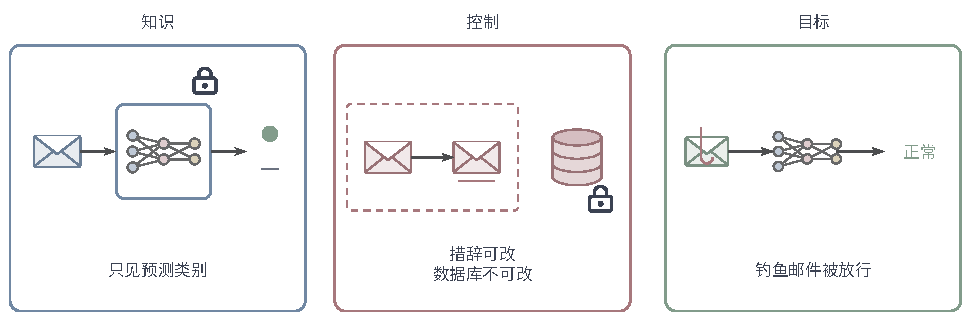
\includegraphics[width=164.405mm]{figures/03-foundations/03-trustworthiness/tikz/trust-threat-model-coordinates/figure.pdf}
  \caption{一次教学威胁模型的压缩视图：仅返回预测类别，可在欺骗目的保持的前提下改写邮件，以钓鱼邮件判正常为成功事件。20次查询是预算而非实验结果。可见信息、可控对象和成功事件不能互推；完整记录还含资产、信任边界、时序、身份与串通范围，无适用取值的字段明确说明。}
  \label{fig:trust-threat-model-coordinates}
\end{figure*}

图~\ref{fig:trust-security-entrypoints}进一步按系统位置标出各类入口（记录内容、更新参数、发布组件、接口输入、提案的行动对象）。确定位置后仍要组合可见信息、修改权限和成功判据，才构成一个完整威胁模型。

\begin{figure*}[htbp]
  \centering
  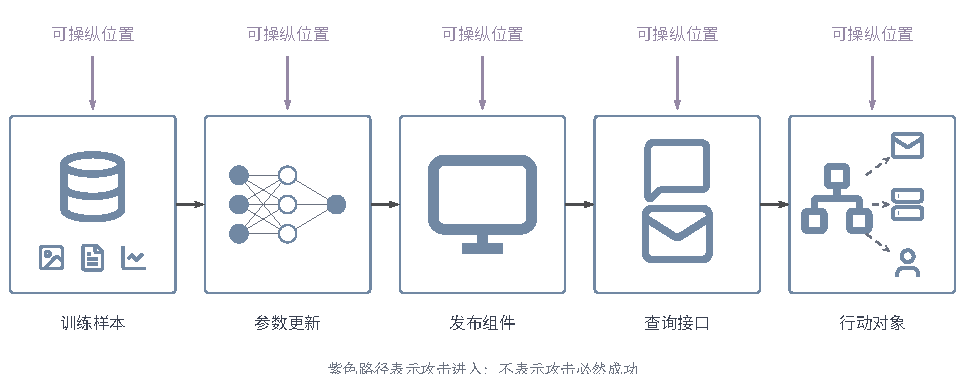
\includegraphics[width=164.600mm]{figures/03-foundations/03-trustworthiness/tikz/security-entrypoints/figure.pdf}
  \caption{攻击入口按可操纵对象定位：记录内容、更新参数、发布组件、接口输入及查询、提案的行动对象。紫色箭头标控制位置，未表示攻击成功；灰色路径标系统阶段联系。同一攻击可经过多个入口，知识、预算和损害目标仍需组合声明。}
  \label{fig:trust-security-entrypoints}
\end{figure*}

\section{脆弱性的评估}
\label{sec:security-evaluation}

给定攻击能力和预算后，脆弱性评估要找出真正能造成损害的路径。为统一口径，先确定评估维度、指标和试验程序（17.2.1），再分别检查预测输入（17.2.2）、受污染训练（17.2.3）、模型与组件供应链（17.2.4）、模型内部机制（17.2.5）、查询接口（17.2.6）和带权限的完整交互执行链（17.2.7）。

六类对象可以串在同一条损害路径上：训练材料里的后门进入参数，部署时的输入触发异常，再经工具执行造成损失。分段测试负责定位薄弱处，关于整条链的系统结论则要核对每一段。白盒搜索、黑盒试探、组件核查和形式化验证都是取证手段，按被测对象能提供的信息和需要证明的性质选用。

\subsection{评估维度与判定标准}
\label{sec:security-risk-assessment}

一个评估设置至少有三个维度：被测对象（查输入、查内部机制还是查工具链）、能力与预算（白盒还是黑盒、查询次数、污染比例）、结果（攻击是否成功、损害多大、正常任务表现如何）。同一个输入入口可以分别在白盒、黑盒和多个预算下测试，因此这些维度必须组合声明。

结果要依次回答四个问题：多少任务被攻破、需要多少次查询或修改、成功后影响多大、正常任务付出什么代价。攻击成功率、预算/污染强度曲线、状态变化与恢复成本、干净任务效用与误拒延迟分别对应这四问。每个数字都要限定它对应的攻击、数据和系统配置；没有说明时不能压成一个笼统的“安全分数”。

\paragraph{可重复的评估程序}

攻击试验按准备、搜索、执行核验和比较四步展开：准备阶段固定测试者能获得的信息；搜索阶段产生候选攻击；执行核验同时检查权限预算和真实系统结果；比较阶段把目标达成、实际损害和正常任务代价分开。后续各类攻击复用这套程序，但材料、搜索方式和核验对象随入口变化。内部核查和形式化验证也可以不构造攻击候选、直接检查计算结构或约束，按实际证据范围报告即可。

\begin{enumerate}
 \item 冻结模型或训练算法版本、预处理、权限配置及正常任务，保存无攻击时的输出或运行状态；将入口、可改对象、可见反馈、预算和成功事件写成可核验条件。
 \item 测试攻击者只接收约定信息，并在预算内生成候选。保存每次查询、反馈、搜索设置和最终提交对象；预算改变时另列试验设置。
 \item 在完整系统中执行有效候选，核对修改范围和最终输出或状态。随机系统重复整个过程，失败、中止及拒绝运行均予保留。
 \item 按预定试验单位汇总成功与损失，并与正常任务比较。防御改变后先复测已知攻击，再让攻击者在同预算内重新搜索，检查适应防御后的结果。
\end{enumerate}

统计单位要特别讲清：若一轮允许改写一封邮件并查询二十次，那么统计单位是“这一预算内的一次完整搜索”，不能把二十次调用当成二十个独立任务。越权归档的成功事件是“授权集合外的邮件状态真的改变”；模型只是提出越权建议，另记为行为偏离。

固定$n$次完整试验，令$s_i\in\{0,1\}$表示第$i$次是否成功，经验攻击成功率（ASR）为$\widehat{\mathrm{ASR}}=n^{-1}\sum_i s_i$。分母包含哪些试验必须预先明确。若指标针对“模型本来能正确处理的任务”，要先冻结这组任务、再算攻击后失败的比例，避免把模型本来就会犯的错算成攻击收益。定向攻击还要核验是否得到了指定结果，而不是“任意错误”都算成功。

\paragraph{攻击结果、损害与证据范围}

成功率要配试验次数和估计误差：独立同分布的完整试验可用二项比例区间；同一任务上的相关搜索要把任务而不是查询当统计单位，重复查询不会增加独立样本量。构造攻击、挑选攻击目标和最终比较应使用职责分开的任务集合，避免只报告在构造阶段就已被攻破的样本。

成功率只数次数，损失量补充严重程度：一次误分类和一次大范围泄露代价不同。令随机元素$\Xi$包含一次完整试验中的任务实例、环境状态、系统随机性和攻击策略自身的随机数；允许策略集合$\mathcal A$中的$a$在抽取$\Xi$之前固定，只能读取威胁模型开放的信息。执行时策略可按获准输入和反馈历史决定下一步（自适性就体现在这个信息接口里，而不能看完整个试验结果再逐个挑选策略）。记损失为$L(a,\Xi)$，规定能力下的最不利风险为
\begin{equation}
 R_{\mathrm{adv}}=\sup_{a\in\mathcal A}
 \mathbb E_{\Xi}[L(a,\Xi)]
 \label{eq:security-adversarial-risk}
\end{equation}
这个上确界是在所有允许策略中比较期望损失。只允许事先选一个固定动作时，$\mathcal A$应限制为常值策略；允许观察当前输入或历史反馈时，把这些观察写进策略接口——这通常会改变风险，不能在$\mathcal A$不变的情况下随意把上确界移进期望。有限次测试只覆盖了部分允许策略，只能提供“已发现风险”的证据，不能精确估计未知攻击的风险上界。

式~\eqref{eq:security-adversarial-risk}是可补偿损失的期望口径。一次泄露或越权就可能造成不可接受后果时，还要看事件概率或尾部：机会约束限制违规事件概率，CVaR 汇总最差尾部的平均损失，它们评价的是同一损失分布的不同方面（可参考\BookChapterRef{chap:decision-theory-and-dynamic-risk}{卷2《数学准备：概率、因果与决策》第6章“策略的价值与优化”}）。明确禁止的状态变化则要靠执行端硬约束：离散时间下，如果执行规则使允许集合内每个状态的所有可能后继状态仍留在集合内，就能从安全初态出发沿轨迹保持安全不变量（可参考\BookChapterRef{chap:control-theory}{卷2《数学准备：概率、因果与决策》第5章“策略的实现与轨迹控制”}）。较低的最坏期望损失替代不了不可补偿的边界。

比较防御时要固定正常任务和资源条件，报告影响范围、恢复成本和任务效用：拒绝所有输入固然能阻断很多攻击，却也取消了服务。有效的比较要说清减少了多少损害、又增加了多少误拒和延迟。

预算改变的是整个过程的成功机会。若每次尝试独立、单次成功概率固定为$p$，则$k$次查询中至少成功一次的概率为$1-(1-p)^k$，随$k$增长；但当攻击者利用失败反馈改写下一次输入时，独立性和固定概率都不再成立，这时应直接把“规定预算内的完整过程”作为一个试验单位。单看每次调用的失败比例，代表不了一个被允许持续试探的服务面临的风险。

防御本身会改变攻击策略：加了关键词过滤，攻击者就改写措辞；加了监控器，监控器本身又可能成为被操纵对象。测试应给攻击者与威胁模型相符的防御知识和试探机会，再比较新一轮搜索结果。旧攻击集用于回归已知问题，不能单独界定改后系统的安全边界。

若要求覆盖规定集合内的全部元素而不仅是“没找到反例”，就要补形式化认证：在输入集合或程序条件下证明性质。证明覆盖的是所写明的集合，能否套用到真实系统仍取决于模型、输入空间和权限假设。例如第~\ref{sec:robustness-certification}节的局部变化界只限定数值扰动，不覆盖训练投毒或工具越权。

\subsection{预测输入的评估}
\label{sec:security-prediction-test}

普通测试只检查给定输入的预测对不对；对抗测试还要在允许修改的范围内主动寻找反例：任务标签应当保持、模型判断却出错。Szegedy 等用输入优化展示了神经网络的这种局部脆弱性，并观察到部分扰动可以在不同网络间迁移，说明在独立测试样本上分类正确，并不覆盖该样本周围所有允许输入的决策行为\scite{szegedy2014intriguing}。

搜索前要准备好原始输入和真实标签、完整的预测接口，以及允许修改集合。白盒额外提供可求梯度的模型信息，黑盒按约定只返回类别或概率。测试始终固定模型、只改输入，先核验预算、合法性和标签保持，再在真实接口上确认候选的预测。

\paragraph{利用输入与输出关系搜索反例}

一个线性打分器就能说明“每个特征只改一点，分数为何会翻”。设$s(\bm{x})=\bm{w}^\top\bm{x}+b$，每个坐标最多改动$\epsilon$。取$\delta_j=\epsilon\operatorname{sign}(w_j)$，所有坐标的改动都朝抬高分数的同一方向，分数共增加$\epsilon\lVert\bm w\rVert_1$。只有当原分数在边界下方、它到边界的差距小于这个可实现的增量时，这一方向才会把分数推过边界；间隔更大时，同样的扰动仍不足以翻转预测。这说明一个机制：单个特征变化小，不保证总分变化小（变化会同向累积）；它只是机制示意，不是说所有模型都必然被攻破。

反向操作可把正分压到负侧。教学评分器$s(\bm{x})=x_1-x_2+0.05$，正分判类别1。原输入$(0.5,0.5)$得0.05；每坐标预算0.1时改成$(0.4,0.6)$得$-0.15$，预测翻转。这个候选只有在“邻域内真实标签仍为1”时才算有效攻击；若改动后真实标签本身已变，就不能把翻转计作攻击成功。

图~\ref{fig:trust-adversarial-perturbation}画出二维情形的允许区域（虚线方框）和候选方向：穿过模型边界只说明预测翻转，候选合法、邻域标签保持仍需独立核验。

\begin{figure}[!htb]
  \centering
  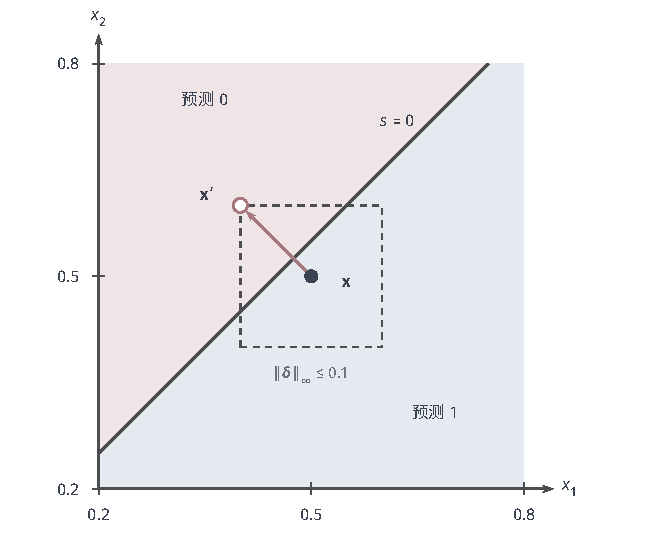
\includegraphics[width=111.404mm]{figures/03-foundations/03-trustworthiness/tikz/trust-adversarial-perturbation/figure.pdf}
  \caption{教学线性评分器中的预算内候选。$(0.5,0.5)$得0.05，$(0.4,0.6)$用扰动$(-0.1,0.1)$、无穷范数0.1得到$-0.15$。浅色为模型预测区，实线为$s=0$，虚线方形为允许集合。翻转只对应模型；邻域真实标签仍为1且候选合法时，才是有效攻击反例。单步构造不保证任意模型的攻击成功。}
  \label{fig:trust-adversarial-perturbation}
\end{figure}

把上面“沿梯度同号方向各走一步”的思路用到损失的局部线性近似上，就得到 Goodfellow 等的\term{快速梯度符号法}（FGSM）。记$\bm g=
\nabla_{\bm x}\ell(f(\bm x),y)$，在无穷范数预算内
\begin{equation}
 \begin{aligned}
 \max_{\|\bm{\delta}\|_\infty\leq\epsilon}
 \bm{g}^{\top}\bm{\delta}
 &=\epsilon\|\bm{g}\|_1,\\
 \bm{\delta}_{\mathrm{FGSM}}
 &=\epsilon\operatorname{sign}(\bm{g}).
 \end{aligned}
 \label{eq:security-fgsm}
\end{equation}
每个坐标都取与梯度同号的端点，就最大化了线性化的损失增量；实际候选还要满足像素取值范围等合法条件。FGSM 只需一次反向传播，但线性化得到的最优扰动不必是原非线性损失的真正最优解\scite{goodfellow2015adversarial}。

对非线性损失，FGSM 的一次近似往往不够。沿用第~\ref{sec:robustness-change-scope}节的允许集合$U(\bm x)$，把寻找高损失输入写成
\[
 \max_{\bm{x}'\in U(\bm x)}\ell(f(\bm{x}'),y).
\]
若$U(\bm x)$是连续数值集合并可计算投影，就沿增大损失方向反复更新、每步投影回允许集合。这样搜到的有效候选是反例；但有限步没搜到，并不认证集合内不存在更强的扰动。

多步搜索每步重算梯度，弥补 FGSM 只做一次线性近似的不足。限定连续数值输入，取无穷范数球$U_\infty(\bm{x})=\{\bm{x}'\in\mathcal X:\lVert\bm{x}'-\bm{x}\rVert_\infty\leq\epsilon\}$，$\mathcal X$为合法输入盒，记$\bm{g}^{(t)}=\nabla_{\bm{x}^{(t)}}\ell(f(\bm{x}^{(t)}),y)$。常用更新为
\begin{equation}
 \bm{x}^{(t+1)}
 =\Pi_{U_\infty(\bm{x})}
 \left[
 \bm{x}^{(t)}
 +\eta\operatorname{sign}(\bm{g}^{(t)})
 \right],
 \label{eq:security-pgd}
\end{equation}
其中$\Pi_{U_\infty(\bm{x})}$是到闭凸允许集合的欧氏投影，轴对齐方盒里就是逐坐标裁剪；$\eta$是步长，初始点可在允许区内随机抽取。这就是 PGD（名称借自投影梯度下降，但这里沿“增大”损失方向走）\scite{madry2018adversarial}。文本等离散集合要另定搜索和可行化方法。随机重启用于探索不同区域、增加迭代用于细化同一条路径，两者不能互相替代；某设置下迭代停滞也不代表找到了最坏输入。

\paragraph{针对防御机制调整搜索}

搜索还要随防御调整：除换初始化和搜索策略外，必要时用迁移攻击；面对随机化或不可微处理则要用专门的搜索机制。一个关键陷阱是\term{梯度掩蔽}（gradient masking）：防御只是让梯度变得难用，决策边界其实依然脆弱。原来的梯度攻击失效，单独不能证明防御有效。

目标函数本身也可能阻碍搜索。Carlini 和 Wagner 评估防御蒸馏时发现概率饱和会让梯度信号失真，于是改用分类前的打分差构造目标。固定图像输入$\bm x\in[0,1]^d$（像素盒只保证数值合法，标签语义另验），针对目标类$k$可写为
\begin{equation}
 \begin{aligned}
 \min_{\bm{x}'\in[0,1]^d}\quad&
 \|\bm{x}'-\bm{x}\|_2^2+c\,h_k(\bm{x}'),\\
 h_k(\bm{x}')={}&
 \max\left\{\max_{j\ne k}
 [z_j(\bm{x}')-z_k(\bm{x}')],-\kappa\right\},
 \end{aligned}
 \label{eq:security-cw}
\end{equation}
其中$z_j$是类别打分，$c>0$权衡扰动大小和攻击项，$\kappa\geq0$指定希望达到的领先间隔。有限$c$的优化结果未必成功：$h_k\leq0$只说明目标类打分不低于其他类，$h_k=-\kappa$才说明至少领先$\kappa$。实践中要搜索$c$，再用真实分类器和平分规则确认输出。数值上搜不动并不等于防御有效——换一个合适的目标函数可能重新暴露出反例\scite{carlini2017evaluating}。

不可微的预处理也可能只是藏起了可用方向而非消除脆弱性。Athalye 等指出应对方法是：前向传播使用真实的防御处理，反向传播时用一个可微近似来搜索；对随机化防御则多次抽取随机变换、用平均损失估计期望梯度。注意候选最终必须在真实防御上成功，在近似模型里成功不算数\scite{athalye2018obfuscated}。

这些攻击改变的环节不同：FGSM/PGD 改变更新步数，CW 改变搜索目标和扰动代价，反向近似与随机变换平均改变取梯度方向的方式；它们可以组合使用，但组合依据是模型接口和防御机制，最终判定始终看候选在真实系统中的结果。

\paragraph{互补搜索与实际输入条件}

单一搜索可能因机制偏置漏掉弱点。AutoAttack 把自动调步长的梯度搜索、边界搜索和无梯度查询搜索组合起来，用互补机制减少手工调参和单一方法造成的漏检\scite{croce2020autoattack}。“免调参”指流程预设了规则，预算仍要声明，对具体防御是否适用仍需检查。

用教学数据核对“多种攻击结果如何合并”：100个样本上两个攻击分别发现12和15个失败，其中8个重合，则并集为$12+15-8=19$个，不能平均成13.5；这组搜索下的鲁棒准确率为$1-19/100=81\%$。其余81个样本只是“尚未找到反例”。在相同样本和允许集合下，真正最坏情况的鲁棒准确率至多为81\%，可能更低。

物理攻击入口改变输入条件：提交的图案经过拍摄、缩放、压缩后，未必还保持数字数组里的攻击效果；只直接输入数组的试验只覆盖数字入口。评价物理攻击要记录成像距离、角度和光照；用随机变换描述这些因素时，要说明变换分布如何代表真实条件。

汇总时先固定集合和预算，只在原本预测正确的样本上按扰动强度计成功率；诱导出指定类别才算定向成功，任意错误算非定向成功。同一样本接受多种搜索时按“是否至少出现一个有效反例”汇总，查询次数不能当独立样本。

\subsection{训练过程的评估}
\label{sec:security-training-test}

训练入口改变了被测过程：输入攻击拿固定模型运行即可，投毒试验则要把受污染材料真正交给学习算法、再检查训练结果。攻击者怎样选择污染内容、学习者采用什么配置，两者都必须固定。

对照试验用完全相同的训练流程：一份用原训练样本，另一份只按规定入口加入或修改污染。采用配对的初始化和超参数、在多个随机种子下重复；留出集既不参与构造污染也不用于挑选“最有利”的防御。若攻击者知识只覆盖一个替代模型，污染先在替代流程中生成、再检验能否迁移到真实训练；不能偷偷用真实梯度，否则就改变了知识条件。

为形式化训练响应，把正常训练样本记成保留索引和重复项的序列$D=((\bm{x}_i,y_i))_{i=1}^n$。令$\mathcal P(D)$为攻击者在规定操作（追加、按索引替换等）和预算下能得到的所有完整训练序列集合；每个$D'\in\mathcal P(D)$都是这些操作作用后的完整序列（不是会合并重复记录的集合）。先限定白盒：攻击者知道$D$、真实算法、目标损失和种子分布，但提交$D'$时不知道本轮实际种子。固定学习规则后学习者按$\mathcal T(D';\xi)$响应，$\xi\sim Q$含初始化、数据顺序等随机性。定向投毒目标为
\begin{equation}
 \begin{aligned}
 \max_{D'\in\mathcal P(D)}\quad&
 \mathbb E_{\xi\sim Q}
 \left[L_{\mathrm{target}}\bigl(\bm{\theta}_{\mathcal T}
       (D',\xi)\bigr)\right],\\
 \text{其中}\quad&
 \bm{\theta}_{\mathcal T}(D',\xi)
 =\mathcal T(D';\xi).
 \end{aligned}
 \label{eq:security-poison-bilevel}
\end{equation}
其中$L_{\mathrm{target}}$按攻击目标选取，值越大表示越接近损害目标，不必等于正常训练的损失。外层选数据、内层$\mathcal T$给出学习者响应，并须明确优化器、超参数、停止准则和多解时如何选择；确定性训练可省去对$\xi$的期望。若种子对攻击者可见、或评价改用最坏种子/分位数，信息条件和统计量都要相应调整。报告要给多个种子的分布，不能用多值$\arg\min$冒充一个确定响应。只知道替代流程时先在替代流程构造$D'$，真实$\mathcal T$只用于迁移评价。这里污染经一次学习影响后续大量预测，与只改一次输入的规避攻击有本质区别。

BadNets 展示了外包训练和模型供应链中的后门风险：让带触发器的样本指向目标类别，同时保持正常输入表现，普通验证集因为不含触发条件而完全发现不了异常。后门还可能随预训练模型迁移到下游任务，所以只检查下游数据来源覆盖不到“模型”这个入口\scite{gu2017badnets}。

“人工核对标签正确”也挡不住所有投毒。Poison Frogs 的\term{干净标签投毒}（clean-label poisoning）保持标签完全合理，却把污染样本在表示空间中放到指定目标附近、悄悄移动分类边界\scite{shafahi2018poison}。这说明标签复核不能替代训练安全审查；其效果依赖表示、训练方式和攻击者的目标知识，不能外推成“少量数据就能控制任意模型”。

两类构造都改训练材料但目标范围不同：BadNets 式后门学的是“触发器$\to$目标类”的联系，让多种输入加触发后同向偏离，验收要看一组触发输入；干净标签投毒往往针对单个目标，用表面正确的样本改变该目标附近的训练约束，验收还要核对预先指定的目标。构造方式和判据都要匹配数据权限与目标范围。

污染的收益必须与无污染训练对照：如果正常模型本来就经常误判目标，不能把污染后的错误全算到攻击头上。应在匹配配置下报告目标错误率、干净性能和初始化变化，并写明污染比例、污染记录是否真的进入训练。后门要同时报“触发时目标成功率”（有效性）和“无触发时性能”（隐蔽性）。

后门指标的分母要小心。固定类别$k$和真实标签非$k$的留出输入，每个样本保留无触发与触发两个版本：配对转移率的主分母取“污染模型在无触发版本不输出$k$”的样本，再算其中触发后转为$k$的比例；更严格时还要求无触发版本原本分类正确。另外单独报告全部非目标样本的触发 ASR、无触发错误率，以及未污染模型在同一配对输入上的结果，才能把“触发转移”和“基线本来就错”分开。跨防御比较时冻结评价样本，按污染预算和触发强度展开，不能只挑最成功的一次训练。

来源、标签和表示异常只提供材料线索，受控投毒才直接检查材料进入学习后的影响，两者要配合。比较不同网络结构时尽量匹配数据、算力和权限，让攻击各自适应对应结构；正常准确率单独回答不了投毒敏感性。若已交付模型无法重跑原训练，就转向内部诊断，并记录“缺少训练样本”这一证据限制。

\subsection{模型与运行组件的供应链评估}
\label{sec:security-supply-chain-test}

交付一个模型不只带来权重，还引入序列化格式、预处理代码、运行依赖和加载权限。供应链检查先冻结版本清单、核验签名和摘要及来源，再在隔离环境记录加载、初始化、预测计算和外部访问。要覆盖文件替换、依赖变更、预处理旁路，以及“来源合法但开发者作恶”——签名排除不了最后一种。来源真实、制品完整、行为安全是三个分别验收的结论。

隔离运行尽量收窄文件、网络、凭据和执行权限，同时检查加载时是否执行未声明代码、访问清单外资源、预处理是否符合冻结版本。出现异常可以定位可疑组件；未见异常也只覆盖当前路径和环境。供应链证据还要与内部机制和完整任务测试合并，才能核实交付物是否真的构成损害路径。

\subsection{模型内部机制的评估}
\label{sec:security-model-test}

内部审查使用计算图、参数、梯度或中间表示来寻找机制或验证行为性质，前提是有相应访问权限；只有查询权时应如实报告结论仅限黑盒范围。审查者获得的内部权限还要与真实攻击者的权限分开声明——前者能力通常更大。

架构名称、层数和参数量决定不了安全性：同一结构用不同数据和参数训练，可能得到完全不同的决策边界或后门。输入测试提供失败候选，内部分析则负责解释失败路径、检验搜索是否充分、并在指定条件下尝试排除反例。

\paragraph{计算路径与局部敏感性的诊断}

诊断计算路径时，先确认预处理、网络各层、随机分支和输出变换都真的在被测执行路径上，再看梯度和激活。单点梯度可以指引搜索方向，但小梯度可能只是激活饱和或被掩蔽，不能当作邻域变化的上界；表示异常也只是候选线索，必须回到预测判断它是否真的实现了攻击目标。

对机制的怀疑可以用受控组件比较检验：在模型副本里替换或移除某组件、其他条件不变，再测攻击和正常任务。例如比较量化前后的真实失败率和梯度可用性，有助于区分“脆弱性被消除”和“只是搜索被阻碍”。副本结果不能冒充原模型结论；第~\ref{chap:trust-interpretability}章的过程解释提供候选机制，安全判断还要补上有效攻击或性质验证。

\paragraph{异常触发机制的诊断}

对已有模型做后门诊断，可以从“是否存在一种触发，能把多类不同输入都推向同一个目标类”入手。Neural Cleanse 对每个目标类反推一个最小触发，用掩码的$\ell_1$范数等量度刻画其大小，再用各类别间的中位数和中位绝对偏差找出异常小的触发\scite{wang2019neuralcleanse}。它把不可穷举的搜索变成可操作诊断，但依赖触发结构和“异常即后门”的假设；输入相关的触发、多个受影响类别、自然类别的不对称都可能削弱判据。

诊断出候选还不等于真有后门：要在独立输入上核验目标类别比例和触发前后变化、检查触发是否可实现；怀疑投毒时还要追溯训练和模型来源。没有找到候选，只说明本次搜索和所假设的结构下没发现异常。

\paragraph{利用计算结构验证行为约束}

内部计算还可以转成约束求解问题：同时规定允许输入、网络计算规则和不希望出现的输出，让求解器判断是否存在满足全部条件的反例。ReLU 网络的线性层给出线性等式，每个神经元激活与否给出分段线性约束。Reluplex 把这些计算规则纳入性质验证，覆盖范围超出有限候选枚举\scite{katz2017reluplex}。

具体地，设原输入正确类别为$y$、类别$j$分数为$z_j(\bm{x}')$、允许集合为$U(\bm{x})$。检查是否存在$\bm{x}'\in U(\bm{x})$和$j\ne y$使$z_j(\bm{x}')\geq z_y(\bm{x}')$，就是找一个至少追平正确类的竞争类。求解出的候选要核验，并按真实平分规则确认误分类；当可靠求解器证明“不可满足”时，才真正排除了集合内全部这类候选。超时和“未知”结果保留为未判定。

也可以沿网络逐层传播区间上下界：只有当每个竞争类别在整个允许集合内的$z_y-z_j$下界都严格为正，才能认证分类不变；下界非正只说明界松，并不代表已经找到攻击。条件和报告方式见第~\ref{sec:robustness-certification}节。结构验证针对给定参数和性质，结论不自动延伸到训练投毒、语义改写或工具权限问题。

\subsection{查询接口的评估}
\label{sec:security-information-test}

查询还能以复制整个服务功能为目标，而不制造单次错误。Tramèr 等指出预测概率等辅助信息实际上给出了关于参数的方程\scite{tramer2016stealing}。以已知的二分类逻辑回归为例：输入$\bm x$、权重$\bm w$、截距$b$，若接口返回类别1的精确概率$p(\bm{x})$，则
\begin{equation}
 \log\frac{p(\bm{x})}{1-p(\bm{x})}
 =\bm{w}^{\top}\bm{x}+b.
 \label{eq:security-model-extraction}
\end{equation}
在预处理已知、概率严格在0和1之间、且查询设计满秩时，$d+1$个独立线性方程恰好确定$d+1$个未知量（$d$维权重加截距）。输出被舍入、隐藏特征或模型更复杂都会改变实际成本；只给类别反馈时虽然没有等式，仍可用来训练替代模型。

一维教学例：$x=0$返回$p=0.5$，$x=1$返回$p=e/(1+e)$。由式~\eqref{eq:security-model-extraction}，第一点给出$b=0$，第二点给出$w+b=1$，故$w=1$。再用没参与求解的输入核验输出、检查接口假设是否成立。可解的关键是“精确概率转成对数几率后是线性方程”，而不是查询本身置信度高。

只给类别反馈、算不了对数几率时，可以改做替代训练：提交允许范围内的输入、收集标签、训练一个替代分类器，再把剩余预算集中到两个模型容易分歧的区域补充样本。方程求解和替代训练都能复制功能，但依赖的反馈和模型假设不同。恢复私人内容仍按上一章的秘密与泄露判据另验。

参数恢复和功能相似要分别测量：两套网络权重不同也可能预测非常接近，只比对权重会漏掉功能复制；而正常常见输入、边界附近和罕见输入上的一致率可能差别很大，评价分布必须声明。预算要同时计查询量、每次反馈的信息量和训练替代模型的成本。

具体试验：让攻击者在规定预算内训练替代模型，用与查询集独立的任务输入测量功能一致率和任务效用，画出随预算变化的曲线。若目标是个人信息或训练内容，则换用第~\ref{sec:privacy-verification}节的成员推断或内容恢复指标——功能一致率本身不构成隐私泄露证据。收益要连同输出粒度、查询限额和已知信息一起报告。

接口的可用性要用专门的资源试验检验：在隔离环境固定并发、输入规模、超时和总预算，比较正常请求与可疑请求的开销、完成率和等待时间。若正常流量本身也触及容量上限要如实报告；只有当少量被允许的请求引起持续异常消耗时，才进一步定位解析、预测或调度路径。复制功能、泄露私人信息和耗尽资源共用同一入口，但成功事件和损失判据各不相同。

\subsection{交互与执行链的评估}
\label{sec:security-interaction-test}

生成式系统必须把“攻击者希望模型说的话”和“系统实际执行的行动”分开。Greshake 等的间接提示注入研究追踪第三方内容如何经检索、工具调用进入上下文，从一个数据来源变成行为操纵入口\scite{greshake2023indirect}。测试必须覆盖来源和授权边界——只检查用户直接输入的恶意要求，覆盖不到这条间接路径。

图~\ref{fig:trust-prompt-injection-boundary}把内容来源和行动授权分开画：越权提案能不能变成实际损害，取决于执行链如何处理提案。

\begin{figure*}[!t]
  \centering
  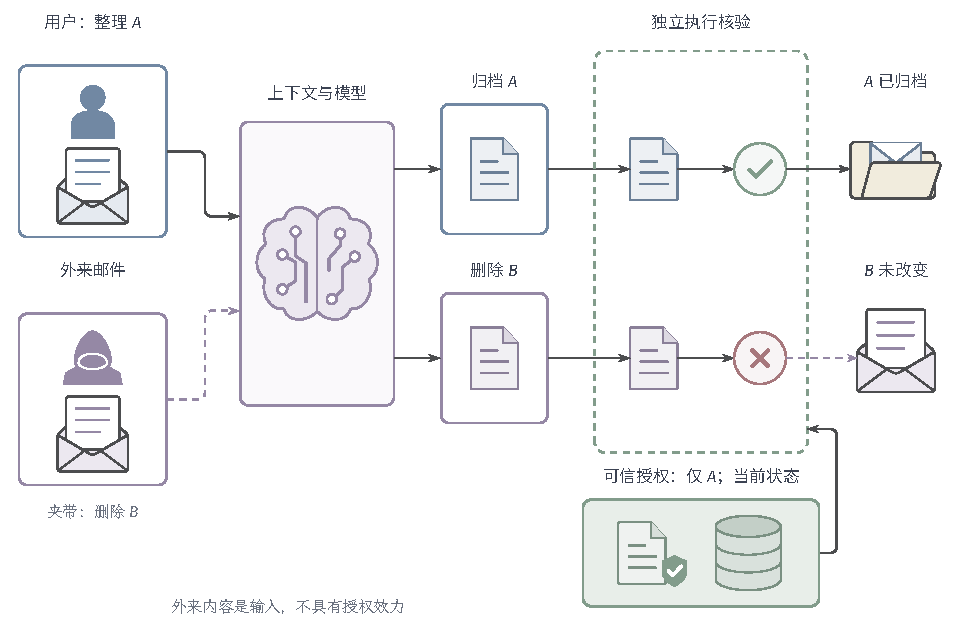
\includegraphics[width=164.600mm]{figures/03-foundations/03-trustworthiness/tikz/prompt-injection-boundary/figure.pdf}
  \caption{第三方邮件影响动作提案的教学情景。用户只授权邮件A，外来内容用虚线夹带删除B要求，模型可能提出归档A及删除B。执行端以可信授权和状态独立检查，允许A而拒绝B，故B不变。这说明防护职责，实际仍需检查旁路、状态变化与损害。}
  \label{fig:trust-prompt-injection-boundary}
\end{figure*}

自动化搜索显著提高了越狱测试的强度。Zou 等用词元梯度筛选能降低攻击代理损失的候选替换、再用前向计算选择离散修改，并研究跨请求和跨模型的迁移\scite{zou2023universal}。代理损失下降仍须经最终行为确认，迁移结果也不覆盖所有版本和系统防护。

AgentDojo 在带工具和真实状态的环境中同时评价两件事：用户的正常任务有没有完成、攻击者指定的偏离有没有发生\scite{debenedetti2024agentdojo}。正常任务指标能区分“真正既保住能力又防住注入”的防御和“一概拒绝工具结果”的偷懒做法。证据仍受环境、权限和攻击集合限制，不能替代真实部署的授权审计。

一轮测试要运行完整任务：按规定位置注入内容，保存读取了什么、提出什么动作提案、执行校验结果和最终状态变化，分别判断用户任务是否完成、攻击目标是否达成。每个任务设无注入对照，再改变来源、权限或预算比较。脱离执行的纯文本试验能测“模型有没有被诱导”，但无法独立测出越权损害。

归档任务可以用集合把四种结果分清。起始时冻结授权动作集合$A$并保存收件箱状态，合法任务需要的动作是$T\subseteq A$，攻击者预定的越权目标是$G$（$G\cap A=\varnothing$）；攻击者只能修改一封待读邮件正文，系统随后产生提案集合$B$、执行器接受集合$C$和最终状态。$B\not\subseteq A$表示模型提案越权，$C\not\subseteq A$表示执行器放行了越权；合法完成要求最终状态等于只执行$T$的预期状态，攻击成功要求状态实现了$G$。四项分计才能区分“未被诱导”“被诱导但被拦下”和“全部拒绝导致任务没做”。

判定工具本身也要核验：关键词可能把“引用恶意指令”和“执行恶意指令”混淆，模型裁判也可能被待评文本操纵。工具类任务优先查外部真实结果（是否真的未授权发送、是否真的越权修改）；无法自动判断的交独立复核，记录标准和不确定性，不用含混分数代替。

\begin{example}[工具权限改变攻击后果]
\label{ex:security-permission}
示例~\ref{ex:security-permission}用两个助手说明工具权限如何改变攻击后果：同一段注入都引出“归档全部邮件”的提案，但甲能直接调用无范围限制的归档接口，乙只拿到本任务授权标识、由执行端复查。同样的文本在甲处变成越权行动、在乙处被权限拦下，因此评价必须区分“模型被诱导”和“是否造成实际损害”。
\end{example}

测试时先把模型和执行器分开以定位授权规则：在隔离环境直接提交正常请求、含越权对象的请求和超数量请求，核对底层状态；再接上受注入的模型重测。前者检验授权规则本身，后者找模型、路由和执行器组合后的旁路。来源标记、路由、持久记忆和重试都要列入路径清单，范围不能停在单轮回答。

\section{攻击防御与损害控制}
\label{sec:security-defense}

防御承接前面定位出的损害路径，按环节干预：来源保护限制材料准入；训练与修复改变学习或参数；输入输出保护约束运行时信息和资源；执行权限控制限制提案变成行动；监测、止损和恢复处理已突破防线的失败。同一条攻击链可被多类措施共同阻断，每类都要有对应试验验证。

用纵深防御理解：恶意邮件可能在输入检查处被拒绝，也可能通过后被模型正确忽略；前两层都失败时，独立执行器仍能拦下越权归档；内容若已写入持久状态还要隔离恢复。这些措施按位置和对象组织，单独采用对抗训练不能证明来源、查询和权限都安全。

\subsection{数据与模型来源的保护}
\label{sec:security-training-defense}

材料准入先核查数据来源、提交主体、标注变更以及模型和处理代码版本。数字签名只有在密钥与身份关联可信且验证通过时才支持来源和完整性；文件摘要要与可信渠道的预期值比对。单个摘要不认证发布者，来源和完整性通过也不证明材料无投毒或后门。

这一步回答“交付物从哪来、拿到后有没有被改”；运行行为是否安全仍需第~\ref{sec:security-supply-chain-test}节的隔离验收。

准入链可独立于预测：登记来源、核验提交主体和数量、新来源先暂存审查、获准对象列入可追踪训练清单。分别用未授权来源、超配额和“合法来源但内容污染”测试：前两类查权限规则，后一类查内容审查能否发现污染，同时报告合法材料误拒率。

合法来源也可能提供异常内容：标签抽查找错误标注，重复度与来源分布找集中提交，表示分析找表面标签正常的污染。每种检查只针对一类线索，需搭配受控污染试验和合法样本误拒评估。

谱特征方法（Spectral Signatures）借候选模型的类别内表示筛查。对某类别表示$\bm h_1,\ldots,\bm h_m$，先减类别均值$\bar{\bm h}$，把各行$\bm h_i-\bar{\bm h}$组成中心化矩阵$H$，取其首个右奇异向量$\bm v_1$作主变化方向，用$|\langle\bm h_i-\bar{\bm h},\bm v_1\rangle|^2$作投影异常分数，按比例或阈值选候选污染、清理后重训\scite{tran2018spectral}。它利用研究所发现后门在表示中的可分离结构，条件含污染比例与表示分离程度，不能认定所有后门都有同样谱异常。

表示筛查需先训练候选模型，宜在隔离环境完成训练与清理再决定材料能否用于后续学习。它形成“借模型改善数据质量”的循环，但仅凭入库字段无法独立完成；审查用途也不赋予候选模型生产准入。

第~\ref{sec:security-model-test}节的诊断只帮助挑选可疑模型、样本和触发线索，不会自动清除异常。修复要记录改了哪些材料、参数或输入规则，再重测触发成功率。

异常只能作调查线索、不能直接批量删除：稀有但合法的群体也可能有异常表示，要考虑第~\ref{chap:trust-fairness}章的代表性问题。修复要同时检查触发是否消失、正常类别和稀有群体性能，避免把安全代价转嫁给特定用户。

\subsection{模型训练与修复}
\label{sec:security-prediction-defense}
\label{sec:security-model-defense}

模型防御直接改变学习规则或参数，按抑制对象分三类：对抗训练降低输入攻击收益，鲁棒聚合限制协作中的恶意更新，已交付模型修复削弱异常机制。三者可组合，但输入训练不自动解决投毒、后门修复也仍需来源审查。

\paragraph{针对输入操纵的训练}

针对输入操纵，可把当前搜到的高损失样本加入训练，近似最小化允许集合内最坏损失。Madry 等用鲁棒优化连接这一目标与攻击搜索\scite{madry2018adversarial}，保护仍限定于允许扰动、搜索强度和训练分布。

做法是极小极大：每个小批次先固定参数，按第~\ref{sec:security-prediction-test}节在允许区域内搜高损失输入，再固定候选更新参数。记参数$\bm\theta$、模型$f_{\bm\theta}$、训练样本$(\bm x,y)\sim\mathcal P_{\mathrm{tr}}$、扰动$\bm\delta$满足$\bm x+\bm\delta\in U(\bm x)$，理想目标为
\begin{equation}
 \min_{\bm\theta}\ \mathbb E_{(\bm x,y)\sim\mathcal P_{\mathrm{tr}}}
 \left[\sup_{\bm\delta:\,\bm x+\bm\delta\in U(\bm x)}
  \ell(f_{\bm\theta}(\bm x+\bm\delta),y)\right].
 \label{eq:security-adversarial-training}
\end{equation}
内层找当前模型的薄弱输入、外层降低这些输入的损失，交替进行。实现中内层搜索步数有限、候选只用于当前更新；参数一变就要重搜，永久复用一组固定攻击样本不等价于该目标。

与固定加噪增强不同，对抗训练的内层随当前参数动态找薄弱点；但内层不充分时模型可能只适应训练见过的攻击模式。最终评估必须包含未参与调参的新攻击，并比较干净性能与不同预算，不能把训练攻击当唯一证据。

第~\ref{sec:robustness-local-enhancement}节的 TRADES（式~\eqref{eq:robustness-trades}）明确权衡正常预测与局部一致性，随机平滑的认证半径（式~\eqref{eq:robustness-smoothing-radius}）在条件成立时给限定集合保证；本章分别用作经验增强和形式保证。像素范数认证不覆盖邮件语义改写，输入扰动训练也不覆盖投毒，换攻击面要重新明确假设。

\paragraph{针对恶意更新的训练规则}

即使参与者身份合法，更新仍可能恶意。鲁棒聚合用对极端值不敏感的规则代替平均。Yin 等分析逐坐标中位数与截尾均值的分布式学习误差，结论需要相应统计与优化条件，尤其要匹配恶意比例和正常更新分布\scite{yin2018byzantine}。

聚合改变参与者向量的合并方式。逐坐标中位数在每一维单独取中位值：教学一维更新$0.9,1.0,1.1,8,9$中后两个由攻击者控制，平均值被拉到4、中位数只有1.1，显示少量极端值对这一维的拉动受限。但高维时各维中位数可能来自不同参与者，正常数据差异也会让更新分散，一维例子不保证聚合向量有用。试验要固定人数和恶意比例，比较攻击后损失、正常收敛和群体损失。

截尾均值先逐维删去规定数量的最大最小值再平均，截掉的数量要匹配威胁条件。伪造大量身份或正常数据高度异质都会破坏比例与集中性前提。第~\ref{sec:privacy-collaborative-computation}节的安全聚合隐藏个体更新，鲁棒聚合则要执行特定运算；组合前必须检查协议能否支持，名称并列不提供联合保证。

\paragraph{训练模型的修复}

有可信后门线索后，可清理受污染材料并从可信起点重训，或直接修订已交付模型。Fine-Pruning 先用干净输入激活剪去低活动神经元、再用干净数据微调其余参数；Liu 等比较单独剪枝、微调与组合，并研究能适应剪枝的攻击，说明修复也要面对攻击者重新选择策略\scite{liu2018finepruning}。

修复需要可信诊断、可信微调数据、正常能力覆盖，以及“异常机制与有用机制可分离”的前提。共用表示时剪枝可能损害正常任务，未测条件中也可能残留后门。验收要重跑触发搜索、已知攻击和保留任务；消除单个触发的效果不能外推到全部未知触发。

安全修复的验收对象是“限定攻击下异常行为消失”，机器遗忘（第~\ref{sec:privacy-unlearning}节）比较的是移除指定记录后的训练结果；两者都改参数但基准不同。依赖查不清或修复不达标时应改用可信数据和可信起点重训，不能继续信任受污染检查点。

\subsection{预测输入与查询输出的保护}
\label{sec:security-information-defense}
\label{sec:security-input-defense}

运行接口有两个防护位置：模型之前的处理决定哪些内容、以什么表示参与计算；交付之后的输出和查询控制决定反馈多少信息、允许尝试多少次。这些措施通常不改训练参数，因此测试必须覆盖包含全部处理的实际接口。

\paragraph{输入检查与可疑请求处置}

格式、类型、长度和范围校验先排除非法输入；语义合法但可疑的请求，可由异常检测、已知触发匹配或独立风险检测决定拒绝、转复核或受限处理。拒绝只是一种处置，不证明攻击识别正确。评价要同时计漏检、正常误拒和接受请求的剩余风险。

去噪、压缩、量化或规范化会改变到达模型的输入，既可能损失任务信息，也可能只是阻碍梯度（梯度掩蔽）。自适应测试要包含完整处理过程，按第~\ref{sec:security-prediction-test}节用反向近似、变换平均或黑盒搜索检查是否只是掩蔽。一种变换有效不证明所有语义保持的攻击都消失。

检索内容和工具返回值应保留来源标记，不能直接提升权限或覆盖配置。恶意短语过滤处理已知模式，角色标记帮助区分指令和数据，但改写和未知模式仍要测。外部材料可能同时含合法步骤和恶意要求，最终行动还要靠下一节的独立授权。

\paragraph{查询输出与资源配额的控制}

减少反馈信息、限制查询次数会提高模型提取或私人信息提取的成本，但也损失正常用途。是否需要正式输出保护按第~\ref{chap:trust-privacy}章判断；参数不公开本身不证明信息不泄露。

反馈粒度直接改变能建立的查询约束：式~\eqref{eq:security-model-extraction}中精确概率给出参数等式，概率区间只给对数几率的区间，仅给类别则只提供边界一侧的信息；查询限额再限制累积量。正常用户也可能因此失去校准概率或批处理能力，返回什么要按业务用途权衡。

固定模型和查询预算，分别用精确概率、有限精度和仅类别反馈训练替代模型，在独立输入上比较功能一致率、再检查正常任务损失，才能区分“减少了信息”和“普遍拖慢了正常使用”。只给类别仍可能逐步逼近决策边界，报告应展示预算与提取效用的关系曲线，而不只是标“是否提供概率”。

模型保密和隐私保护对象不同：差分隐私限制一条记录或一个用户的变化对发布分布的影响，却允许发布总体规律，因此模型功能仍可能被近似复制；隐藏结构也不提供训练样本隐私保护。接口设计要先明确是保护个人信息、商业模型还是安全规则知识，再设对应判据。

改接口后按第~\ref{sec:security-information-test}节复测同一预算下的提取收益，并记录正常限流、精度损失和延迟。若多账户、多会话在攻击权限内，配额必须按同一身份边界计量——单会话限额不等于完整攻击预算。

资源配额可限制输入大小、并发数、生成长度、工具调用次数和任务时长，并隔离租户队列。配额要覆盖完整任务和可识别主体，否则靠重试或多会话就能累积超限。测试要同时检查异常消耗和长文本、批处理等合法需求的损失。

\subsection{行动执行中的权限控制}
\label{sec:security-execution-defense}

第~\ref{sec:alignment-intervention-execution}节已把模型输出限定为动作提案、由独立执行器复核对象参数和状态。本节进一步检验攻击者能否绕过这些规则，范围包括可控身份、内容、调用顺序和反馈；仅有一个检查步骤存在，不足以支持安全结论。

权限先缩到任务所需：摘要任务不需要删除权限，读指定文档不需要访问整个私有目录。测试再覆盖伪造身份标识、在批量参数里夹带越权对象、检查与执行之间被篡改状态、用多账户或连续低权限动作绕过单账户上限等路径。沙箱和结构化参数的作用取决于这些路径受到什么约束，名字不能替代隔离边界。

多层措施还要检查共同弱点：如果过滤、行为评判和授权用的是同一个能被文本操纵的模型，层数再多风险也未必明显下降。设计要追踪共享信息，并检查各层失效是否相互独立。

测试顺序：先直接对执行器提交伪造主体、越权或重复对象、超量批量和“状态已变”的请求，核对底层状态；再把同样条件放回受提示注入的完整交互。前者检验授权规则本身，后者检查模型、路由和执行器组合后有无旁路。每轮都核对底层状态和正常完成情况；文本被拒绝只是行为结果，越权对象确实没有状态变化才支持相应的执行边界。

来源保留同样适用于检索增强：网页内容可以提供任务事实，却不能更改工具授权；加引号或“不可信”标记只是给模型一个区分信号，仍需模型正确理解。外部检查应在模型忽略该信号时依然限制越权。对不可逆动作的复核界面要列出具体对象和后果，使被批准的行动清晰可辨。

\subsection{攻击监测与损害恢复}
\label{sec:security-recovery}

残余风险要求监测与响应衔接。异常的查询密度、资源消耗、工具使用范围、连续拒绝、版本变化和外部数据流向都能提供线索，再结合系统状态和独立记录判断是否处置。模型自称“未受攻击”不能代替证据，误报和漏报要实际演练计量。

响应措施随传播位置选择：暂停任务和后续工具调用、撤销会话凭据、隔离数据或模型版本，必要时切到受限功能或已验证版本。外发正在发生时先关出口，模型被污染时停止该版本继续决策；只拒绝当前输入清不掉参数或记忆中的污染。

检测可能晚于部分损害。限制动作规模、保存可恢复状态、撤权和停止后续操作可以缩小影响，但这些能力要实际测量。文件恢复收不回已经外发的信息，停止后续行动也撤销不了已经发生的不可逆操作。

可做隔离演练：先保存状态，运行一条“错误修改邮件标签”的教学轨迹，在预定时刻触发检测，检查后续动作是否停止、权限是否撤销、标签是否恢复，并记录从检测到停止的时长、受影响对象、恢复状态和残余损失。已经外发的信息只能检查后续传播是否受限，本地删日志不等于收回信息。演练回答的是“发现失效后还能控制什么”，不替代原来的攻击判定。

还要保全能区分模型错误、提示注入和授权配置问题的证据；日志可能含敏感输入，按第~\ref{chap:trust-privacy}章限制访问和保留期限。只替换模型却保留注入入口、或只删文档却不检查记忆和派生状态，都可能留下继续触发的路径。恢复范围必须沿信息传播确定。

处置后回到第~\ref{sec:security-evaluation}节，同时复测正常任务、已知攻击和适应新防御的新搜索，报告在规定能力预算下被限制的损害和未覆盖条件。

重新开放还要有退出门槛：按冻结清单和传播路径逐项核对受影响资产、依赖和派生状态，无法确认的引用列为未闭合项；恢复版本必须来自可信基线或可复核重建；相关凭据、配置、模型、记忆和派生状态完成轮换、清理或隔离；原入口和已知旁路要在规定能力预算下通过回归、自适应复测和底层状态核验，正常任务达到预设最低性能，不可逆的残余损失单独登记。门槛不过就保持隔离或受限服务并保留可回退版本；全部通过也只支持在同一威胁模型下逐步恢复权限，不排除未知攻击。

图~\ref{fig:trust-defense-in-depth}把准入、模型复核、接口、独立授权和监测恢复放到传播路径上：来源检查能拦未授权材料，但不保证发现合法来源的污染；格式合法的注入可能穿过输入和模型，授权仍要独立限制对象；恢复负责处理既有影响，与事前阻断分别记录。

\begin{figure*}[htbp]
  \centering
  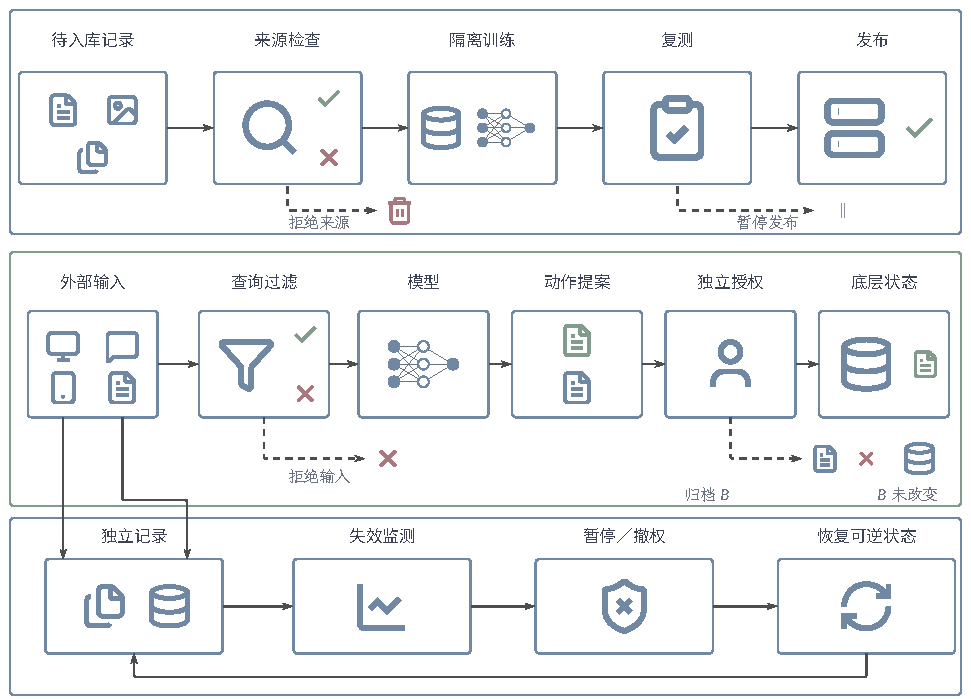
\includegraphics[width=164.600mm]{figures/03-foundations/03-trustworthiness/tikz/defense-in-depth/figure.pdf}
  \caption{纵深防御在训练与运行路径上的分工。未授权来源止于准入，异常候选模型暂不发布，但来源通过不证明内容无污染。合法格式的外部注入可到模型并提出归档B，独立授权拒绝越权对象后B不变。监测用独立记录和底层状态，失效后暂停、撤权及恢复可逆状态；外发信息不能据此收回。阻断依赖相应检查触发，未保证全部攻击可发现，也未假定各层失效独立。}
  \label{fig:trust-defense-in-depth}
\end{figure*}

\FloatBarrier
\Needspace{4\baselineskip}
\section{本章小结}
\label{sec:security-summary}

第一条结论：邮件系统的安全判断已从“单次预测对不对”扩展到信息路径和行动路径。攻击类型描述操纵操作，完整性、机密性、可用性描述损害，威胁模型固定可见信息、可改对象和尝试预算。沿这些条件核验时，预测出错、越权提案和实际损害必须分别记录，才能看出保护在哪一环失效或生效。

第二条：输入反例、配对投毒训练、供应链隔离、内部机制分析、查询收益测量和完整状态测试各提供一种证据，合起来限定已发现脆弱性的范围。单次搜索失败、架构名称和干净成绩都不能取代这些检查；成功率只有连同预算、损害、正常代价和覆盖范围一起报告，才支持防御比较。

第三条：防御选择由薄弱位置决定——来源审查不能自行消除参数后门，训练不能代替配额与授权，过滤不能自行清理持久状态。组合数据、模型、接口和执行保护后，还要在同条件下开放新一轮搜索；监测与恢复决定突破后的损失边界，外泄信息和可逆的状态修改必须分开验收。

第四条与全卷呼应：第~\ref{chap:trust-alignment}章讨论无外部攻击时的目标偏离，本章增加有目的的操纵——攻击者可以利用预测误差、环境变化、信息泄露和权限缺口使保护失效。因此要在同一系统、同一明确攻击能力内复核前面各章的性质；改善其中一项，仍须检查其他损害路径。

\paragraph{扩展阅读}

Madry等的鲁棒优化与Athalye等的自适应攻击，可用来对照防御训练与评估：前者把扰动范围纳入训练，后者区分梯度搜索受阻与脆弱性消除。继续阅读时，始终分开经验失败和形式化认证\scite{madry2018adversarial,athalye2018obfuscated}。

检索及工具系统可沿间接提示注入与AgentDojo继续阅读：前者追踪第三方内容进入行为链，后者同时判用户任务和攻击目标。比较时保留输出提案、执行端接受动作及最终状态这三个层次\scite{greshake2023indirect,debenedetti2024agentdojo}。
